\documentclass[11pt,a4paper]{report}
\usepackage{tikz,graphicx}
\usepackage{titlesec}
\usepackage[utf8]{inputenc}
\usepackage[left=3.2cm,right=2.6cm]{geometry}
\usepackage{calc}
\usepackage{eso-pic}
\usepackage[section]{placeins}
\usepackage{float}
\usepackage[hidelinks]{hyperref}
\usepackage{listings}

\setlength{\topmargin}{0in}
\begin{document}


\title{Analysis of CPU Scheduling Algorithms}


\author{Kashish Srivastava (185014)\\
        \and 
        Dipesh Kumar (185015)\\
        \and
        Akash Rana (185034)
}

\titleformat{\chapter}{\bfseries\huge\centering}{}{0pt}{}{\huge}
\titlespacing*{\chapter}{0pt}{-60pt}{20pt}
\setlength{\parindent}{2em}
\setlength{\parskip}{1em}

\newenvironment{myindentpar}[1]
  {\begin{list}{}
          {\setlength{\leftmargin}{#1}}
          
  }
  {\end{list}}
\date{July 2020}

\pagestyle{plain}

\begin{titlepage}
    \begin{center}

        \Huge{\textbf{Analysis of CPU Scheduling Algorithms}}
 
        \vspace{5pt}
        
        \normalsize
       
        \vspace{5pt}
        
        Operating Systems\\
        CSD-222

    
        \vspace{10pt}
        
\includegraphics[width=0.4\textwidth]{./img/logo.png}
        
        \vspace{15pt}
        \textit{Submitted by:}\\
            Kashish Srivastava (185014)\\
            Dipesh Kumar (185015)\\
            Akash Rana (185034)
        \vspace{5pt}
 
        CSE (4 Year) : 
        4\textsuperscript{th} Semester
 
        \vspace{1cm}
 
        Under the guidance of
        
        \vspace{5pt}
        
        \textbf{Dr. Pradeep Singh }\\
		\large
		Assistant Professor\\ Department of Computer Science and Engineering\\
		National Institute of Technology, Hamirpur\\
		
      
    \end{center}
\end{titlepage}


\tableofcontents

\chapter{Introduction}
\vskip 1cm
\hspace*{\parindent}This document is a report for the individual project ``Simulation of various CPU scheduling algorithms and analysing the behaviour of each scheduler". CPU scheduling is a process which allows one process to use the CPU while the execution of another process is on hold(in waiting state) due to unavailability of any resource like I/O etc, thereby making full use of CPU. The aim of CPU scheduling is to make the system efficient, fast and fair.\\ 
\vskip 1cm
\begin{figure}[H]
\centering
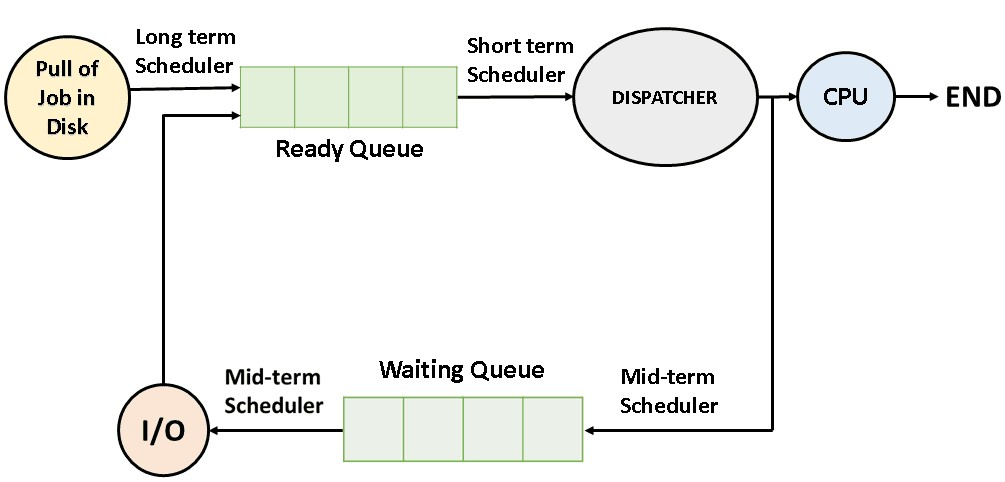
\includegraphics[scale=0.5]{./img/cpu.jpg}
\caption{Cpu scheduling}
\end{figure}

The project is an attempt to differentiate the behaviour of each scheduler with the statistical approach. In this project we performed each CPU scheduling and compared them on the basis of their completion time,throughput,average job elapsed time and average job waiting time during the process. It also discusses the complexity of the written code as instructed.


\chapter{Software requirement and specification}

\subsection*{Python(3.7.6)}
{Python is an interpreted, high-level, general-purpose programming language. Created by Guido van Rossum and first released in 1991, Python's design philosophy emphasizes code readability with its notable use of significant whitespace.}

{\subsection*{Python-dateutil(2.8.1)}
{The dateutil module provides powerful extensions to the standard datetime module, available in Python.}

\subsection*{matplotlib(3.2.2)}
{Matplotlib is a comprehensive library for creating static, animated, and interactive visualizations in Python.}

\subsection*{cycler(0.10.0)}
{A single entry Cycler object can be used to easily cycle over a single style.}


\subsection*{numpy(1.19.0)}
{NumPy is the fundamental package for scientific computing in Python. It is a Python library that provides a multidimensional array object, various derived objects (such as masked arrays and matrices).}

\subsection*{Kiwisolver(1.2.0)}
{Kiwisolver is an efficient C++ implementation of the Cassowary constraint solving algorithm. Kiwi is an implementation of the algorithm based on the seminal Cassowary paper.}

\subsection*{pyparsing(2.4.7)}
{Pyparsing is a mature, powerful alternative to regular expressions for parsing text into tokens and retrieving or replacing those tokens.}

\subsection*{six(1.15.0)}
{Six provides simple utilities for wrapping over differences between Python 2 and Python 3. It is intended to support codebases that work on both Python 2 and 3 without modification.}
}

\chapter{Usage}

Install Python 3.7.6 and then install all packages mentioned in 'requirements.txt' in root folder by:

	\begin{lstlisting}[ language=Python ]
		python -m pip install -r requirements.txt
		
	\end{lstlisting}

After Installing all the packages run the main script with command:

\begin{center}
	\begin{lstlisting}[ language=Python ]
		python main.py
		
	\end{lstlisting}
\end{center}


\begin{figure}[H]
\begin{center}
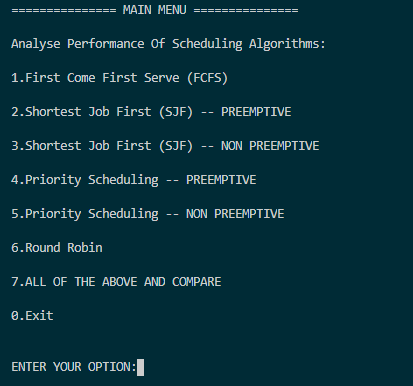
\includegraphics{./img/main.PNG}
\caption{Main Menu}
\label{fig}
\end{center}
\end{figure}


\chapter{Theory}

\hspace*{\parindent}CPU scheduling is a process which allows one process to use the CPU while the execution of another process is on hold(in waiting state) due to unavailability of any resource like I/O etc, thereby making full use of CPU. The aim of CPU scheduling is to make the system efficient, fast and fair.

Whenever the CPU becomes idle, the operating system must select one of the processes in the ready queue to be executed. The selection process is carried out by the short-term scheduler (or CPU scheduler). The scheduler selects from among the processes in memory that are ready to execute, and allocates the CPU to one of them.

\section{Types of CPU Scheduling}

CPU scheduling decisions may take place under the following four circumstances:

\begin{enumerate}
	\item When a process switches from the running state to the waiting state(for I/O request or invocation of wait for the termination of one of the child processes).
    \item When a process switches from the running state to the ready state (for example, when an interrupt occurs).
    \item When a process switches from the waiting state to the ready state(for example, completion of I/O).
    \item When a process terminates.
\end{enumerate}
    

In circumstances 1 and 4, there is no choice in terms of scheduling. A new process(if one exists in the ready queue) must be selected for execution. There is a choice, however in circumstances 2 and 3.

When Scheduling takes place only under circumstances 1 and 4, we say the scheduling scheme is non-preemptive; otherwise the scheduling scheme is preemptive.

\section{Preemptive Scheduling}
\hspace*{\parindent}In this type of Scheduling, the tasks are usually assigned with priorities. At times it is necessary to run a certain task that has a higher priority before another task although it is running. Therefore, the running task is interrupted for some time and resumed later when the priority task has finished its execution.

\section{Non-Preemptive Scheduling}
\hspace*{\parindent}Under non-preemptive scheduling, once the CPU has been allocated to a process, the process keeps the CPU until it releases the CPU either by terminating or by switching to the waiting state.
It is the only method that can be used on certain hardware platforms, because it does not require the special hardware(for example: a timer) needed for preemptive scheduling.

\section{Scheduling Algorithms}
\subsection*{First Come First Serve Scheduling}
\hspace*{\parindent}In the "First come first serve" scheduling algorithm, as the name suggests, the process which arrives first, gets executed first, or we can say that the process which requests the CPU first, gets the CPU allocated first. First Come First Serve, is just like FIFO(First in First out) Queue data structure, where the data element which is added to the queue first, is the one who leaves the queue first. This is used in Batch Systems. It's easy to understand and implement programmatically, using a Queue data structure, where a new process enters through the tail of the queue, and the scheduler selects process from the head of the queue. FCFS provides an efficient, simple and error-free process scheduling algorithm that saves valuable CPU resources. It uses nonpreemptive scheduling in which a process is automatically queued and processing occurs according to an incoming request or process order. FCFS derives its concept from real-life customer service.

\subsection*{Shortest Job First Scheduling}
\hspace*{\parindent}Shortest job next (SJN), also known as shortest job first (SJF) or shortest process next (SPN), is a scheduling policy that selects for execution the waiting process with the smallest execution time. SJN is a non-preemptive algorithm. Shortest remaining time is a preemptive variant of SJN.

Shortest job next is advantageous because of its simplicity and because it minimizes the average amount of time each process has to wait until its execution is complete. However, it has the potential for process starvation for processes which will require a long time to complete if short processes are continually added. Highest response ratio next is similar but provides a solution to this problem using a technique called aging.

Another disadvantage of using shortest job next is that the total execution time of a job must be known before execution. While it is impossible to predict execution time perfectly, several methods can be used to estimate it, such as a weighted average of previous execution times.

Shortest job next can be effectively used with interactive processes which generally follow a pattern of alternating between waiting for a command and executing it. If the execution burst of a process is regarded as a separate "job", past behaviour can indicate which process to run next, based on an estimate of its running time.

\subsection*{Priority Scheduling}
\hspace*{\parindent}Priority scheduling is a scheduling system commonly used in real-time systems. With fixed priority preemptive scheduling, the scheduler ensures that at any given time, the processor executes the highest priority task of all those tasks that are currently ready to execute.

The preemptive scheduler has a clock interrupt task that can provide the scheduler with options to switch after the task has had a given period to execute—the time slice. This scheduling system has the advantage of making sure no task hogs the processor for any time longer than the time slice. However, this scheduling scheme is vulnerable to process or thread lockout: since priority is given to higher-priority tasks, the lower-priority tasks could wait an indefinite amount of time. One common method of arbitrating this situation is aging, which gradually increments the priority of waiting processes and threads, ensuring that they will all eventually execute. Most real-time operating systems (RTOSs) have preemptive schedulers. Also turning off time slicing effectively gives you the non-preemptive RTOS.

\subsection*{Round Robin Scheduling}
\hspace*{\parindent}Round-robin (RR) is one of the algorithms employed by process and network schedulers in computing. As the term is generally used, time slices (also known as time quanta) are assigned to each process in equal portions and in circular order, handling all processes without priority (also known as cyclic executive). Round-robin scheduling is simple, easy to implement, and starvation-free. Round-robin scheduling can be applied to other scheduling problems, such as data packet scheduling in computer networks. It is an operating system concept.



\chapter{First Come First Serve (FCFS)}


\begin{lstlisting}[columns=fullflexible,caption=FCFS Source Code,breaklines=true,postbreak=\mbox{\textcolor{red}{$\hookrightarrow$}\space}]
import matplotlib.pyplot as plt

plt.style.use('fivethirtyeight')

## Finds waiting time for each process
def findWaitingTime(processes,  burst_time, waiting_time, arrival_time):  
    service_time = [0] *len(processes) 
    service_time[0] = 0
    waiting_time[0] = 0
    for i in range(1, len(processes)):  
           
        service_time[i] = (service_time[i - 1] +  burst_time[i - 1])  
  
        waiting_time[i] = service_time[i] - arrival_time[i]  
        if (waiting_time[i] < 0): 
            waiting_time[i] = 0
      

#Finds Turn Around Time for All processes
def findTurnAroundTime(processes, burst_time, waiting_time, turn_around_time):  
    for i in range(len(processes)): 
        turn_around_time[i] = burst_time[i] + waiting_time[i]  
  
  
#Returns waiting,turn around, completion time for each process
def findavgTime(processes,  burst_time, arrival_time):  

    waiting_time = [0] *len(processes)
    turn_around_time = [0] *len(processes) 
    findWaitingTime(processes,  burst_time, waiting_time, arrival_time)  
    findTurnAroundTime(processes,  burst_time, waiting_time, turn_around_time)  

    total_wt = 0
    total_turn_around_time = 0
    compl_time = [0]*len(processes)
    for i in range(len(processes)): 
  
        total_wt = total_wt + waiting_time[i]  
        total_turn_around_time = total_turn_around_time + turn_around_time[i]  
        # Calculate completion time

        compl_time[i] = turn_around_time[i] + arrival_time[i] 

    return waiting_time , turn_around_time ,compl_time


def plot_graph(processes,waiting_time,compl_time,turn_around_time):

    plt.plot(processes,waiting_time,label = "Waiting time")
    plt.plot(processes,compl_time,label = "Completion time")
    plt.plot(processes,turn_around_time,label = "Turnaround Time")
    plt.text(4,2,'Throughput = %.5f'  % (len(processes)/ compl_time[len(processes)-1]))
    plt.title("First Come First Serve Algo")
    plt.xlabel("Processes")
    plt.ylabel("Time Units")
    plt.legend()
    plt.savefig('./output/FCFS_output.png')
    plt.show()



def print_details(processes,waiting_time,turn_around_time,compl_time,burst_time,arrival_time):
      
    print("Processes   Burst Time   Arrival Time     Waiting",  
          "Time   Turn-Around Time  Completion Time \n") 
    for i in range(len(processes)):
        print(" ", processes[i] , "\t\t", burst_time[i], "\t\t", arrival_time[i],  
              "\t\t", waiting_time[i], "\t\t ", turn_around_time[i], "\t\t ", compl_time[i])  
  
    print("Average waiting time = %.5f "%(sum(waiting_time) /len(processes))) 
    print("\nAverage turn around time = ", sum(turn_around_time) / len(processes))  
    print('\nThroughput = ', len(processes)/ compl_time[len(processes)-1])


# driver function

def fcfs():
 
    processes = []
    burst_time = []
    arrival_time = []
    #breakpoint
    with open('./inputs/FCFS.txt','r') as  f:
        f.readline()
        for line in f.readlines():
            process , burst , arrival = (line.split(" "))
            processes.append(process)
            burst_time.append(int(burst))
            arrival_time.append(int(arrival))

    #returned waiting time and turn around time
    waiting_time , turn_around_time, compl_time = findavgTime(processes,  burst_time, arrival_time)
    
    #print details about data
    print_details(processes,waiting_time,turn_around_time,compl_time,burst_time,arrival_time)

    #plotting 
    plot_graph(processes,waiting_time,compl_time,turn_around_time)
    plt.close(fig='all')

if __name__ =="__main__": 
    fcfs()
\end{lstlisting}

\begin{figure}[H]
	\centering
	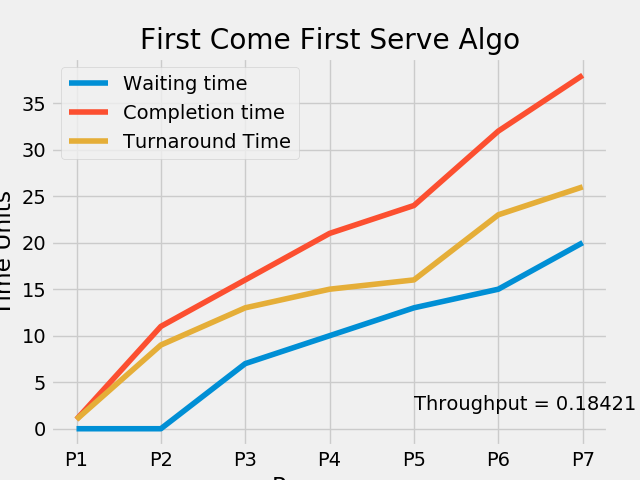
\includegraphics[scale=0.8]{./img/FCFS_output.png}
	\caption{FCFS output values.}
\end{figure}

\begin{figure}[H]
	\centering
	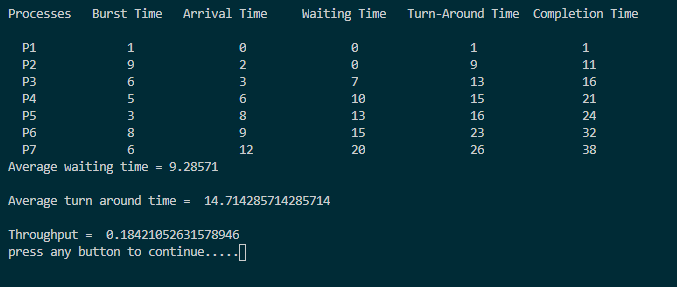
\includegraphics[scale=0.8]{./img/fcfs_out.PNG}
	\caption{FCFS output values.}
\end{figure}


\chapter{Shortest Job First(SJF)}
\section{SJF(Preemptive)}
\begin{lstlisting}[columns=fullflexible,caption=SJF (Preemptive) Source Code,breaklines=true,postbreak=\mbox{\textcolor{red}{$\hookrightarrow$}\space},]
import matplotlib.pyplot as plt;

plt.style.use('fivethirtyeight')
	
def findWaitingTime(processes, n, wt):  
	rt = [0] * n 
	for i in range(n):  
		rt[i] = processes[i][1] 
	complete = 0
	t = 0
	minm = 999999999
	short = 0
	check = False
	
	while (complete != n): 
		for j in range(n): 
			if ((processes[j][2] <= t) and 
				(rt[j] < minm) and rt[j] > 0): 
				minm = rt[j] 
				short = j 
				check = True
		if (check == False): 
			t += 1
			continue
				
		rt[short] -= 1
		minm = rt[short]  
		if (minm == 0):  
			minm = 999999999
		if (rt[short] == 0):  
	
			complete += 1
			check = False
			fint = t + 1
			wt[short] = (fint - processes[short][1] -processes[short][2]) 
	
			if (wt[short] < 0): 
				wt[short] = 0
		t += 1


def findTurnAroundTime(processes, n, wt, tat):  
	
	for i in range(n): 
		tat[i] = processes[i][1] + wt[i]  


	
def findavgTime(processes, n):  
	wt = [0] * n 
	tat = [0] * n  
	findWaitingTime(processes, n, wt)  
	findTurnAroundTime(processes, n, wt, tat)  
	compl_time = []
	for i in range(n):
			compl_time.append(tat[i]+processes[i][2])
	return wt, tat,compl_time


def print_data(processes,w_time,tat_time,compl_time,n):
	
	print("Processes\t\tBurst Time\t\tWaiting",  
					"Time\t\tTurn-Around Time\t\tArrival Time\t\tCompletion Time" )
	for i in range(n): 
	
		print(" ", processes[i][0], "\t\t\t",  
					processes[i][1], "\t\t\t",  
					w_time[i], "\t\t\t", tat_time[i],'\t\t\t\t',processes[i][2],'\t\t\t',compl_time[i]) 
	
	print("\nAverage waiting time = %.5f "%(sum(w_time) /n) ) 
	print("Average turn around time = ", sum(tat_time) / n)  
	print("Throughput  =  ",n/max(compl_time))


def  plot_graph(processes,waiting_time,compl_time,turn_around_time):

	plt.plot(processes,waiting_time,label = "Waiting time")
	plt.plot(processes,compl_time,label = "Completion time")
	plt.plot(processes,turn_around_time,label = "Turnaround Time")
	plt.text(4,2,'Throughput = %.5f'  % (len(processes)/ compl_time[len(processes)-1]))
	plt.title("SJF PREEMPTIVE")
	plt.xlabel("Processes")
	plt.ylabel("Time Units")
	plt.legend()
	plt.savefig('./output/SJF_P_output.png')
	plt.show()



def sjf_p():
	process_data = []
	
	with open('./inputs/SJF_P.txt','r') as  f:
		f.readline()
		for line in f.readlines():
			temporary = []
			process , burst , arrival = (line.split(" "))
			temporary.extend([process, int(burst), int(arrival)])
			process_data.append(temporary)
	n = len(process_data)
	w_time,tat_time,compl_time =  findavgTime(process_data, n) 
	print_data(process_data, w_time, tat_time,compl_time,n)
	plot_graph([p[0] for p in process_data],w_time,compl_time,tat_time)
	plt.close(fig='all')

# Driver code  
if __name__ =="__main__": 
	sjf_p()


\end{lstlisting}
{\begin{figure}[H]
	\centering
	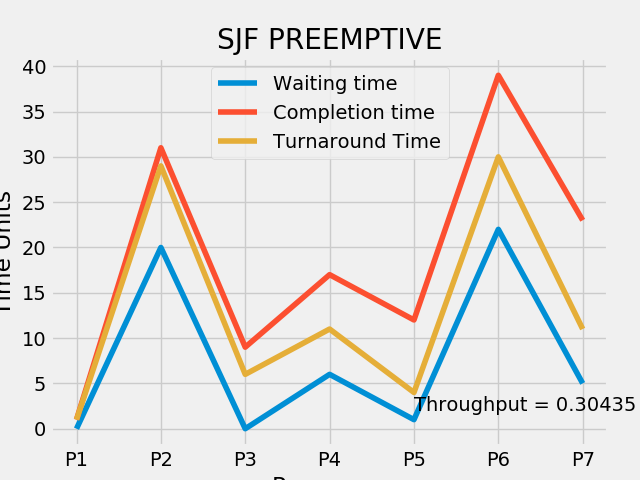
\includegraphics[scale=0.75]{./img/SJF_P_output.png}
	\caption{SJF(Preemptive) output values.}
\end{figure}}

{\begin{figure}[H]
	\centering
	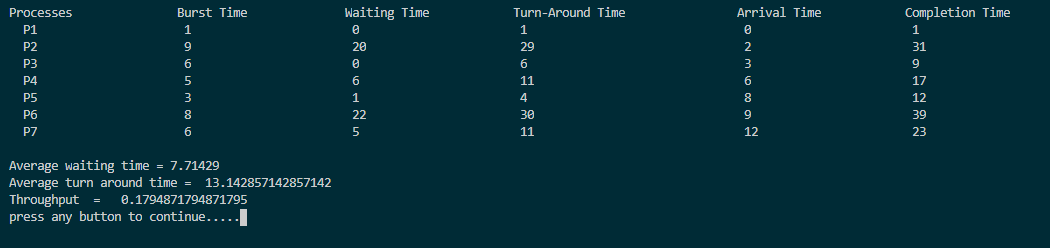
\includegraphics[scale=0.5]{./img/sjf_p_out.PNG}
	\caption{SJF(Preemptive) output values.}
\end{figure}}

\section{SJF(Non-Preemptive)}
\begin{lstlisting}[columns=fullflexible,caption=SJF (Non-Preemptive) Source Code,breaklines=true,postbreak=\mbox{\textcolor{red}{$\hookrightarrow$}\space},]
import matplotlib.pyplot as plt

plt.style.use('fivethirtyeight')



def schedulingProcess(  process_data):
	start_time = []
	exit_time = []
	s_time = 0
	process_data.sort(key=lambda x: x[1])
	'''
	Sort processes according to the Arrival Time
	'''
	for i in range(len(process_data)):
		ready_queue = []
		temp = []
		normal_queue = []

		for j in range(len(process_data)):
			if (process_data[j][1] <= s_time) and (process_data[j][3] == 0):
				temp.extend([process_data[j][0], process_data[j][1], process_data[j][2]])
				ready_queue.append(temp)
				temp = []
			elif process_data[j][3] == 0:
				temp.extend([process_data[j][0], process_data[j][1], process_data[j][2]])
				normal_queue.append(temp)
				temp = []

		if len(ready_queue) != 0:
			ready_queue.sort(key=lambda x: x[2])
			'''
			Sort the processes according to the Burst Time
			'''
			start_time.append(s_time)
			s_time = s_time + ready_queue[0][2]
			e_time = s_time
			exit_time.append(e_time)
			for k in range(len(process_data)):
				if process_data[k][0] == ready_queue[0][0]:
					break
			process_data[k][3] = 1
			process_data[k].append(e_time)

		elif len(ready_queue) == 0:
			if s_time < normal_queue[0][1]:
				s_time = normal_queue[0][1]
			start_time.append(s_time)
			s_time = s_time + normal_queue[0][2]
			e_time = s_time
			exit_time.append(e_time)
			for k in range(len(process_data)):
				if process_data[k][0] == normal_queue[0][0]:
					break
			process_data[k][3] = 1
			process_data[k].append(e_time)

	calculateTurnaroundTime(  process_data)
	calculateWaitingTime(  process_data)

	waiting_time = [p[6] for p in process_data]
	turn_around_time = [p[5] for p in process_data]
	compl_time = [p[4] for p in process_data]
	return waiting_time,turn_around_time,compl_time


def calculateTurnaroundTime(  process_data):
	total_turnaround_time = 0
	for i in range(len(process_data)):
		turnaround_time = process_data[i][4] - process_data[i][1]
		'''
		turnaround_time = completion_time - arrival_time
		'''
		total_turnaround_time = total_turnaround_time + turnaround_time
		process_data[i].append(turnaround_time)
	

def calculateWaitingTime(  process_data):
	total_waiting_time = 0
	for i in range(len(process_data)):
		waiting_time = process_data[i][5] - process_data[i][2]
		'''
		waiting_time = turnaround_time - burst_time
		'''
		total_waiting_time = total_waiting_time + waiting_time
		process_data[i].append(waiting_time)
	



def printData(  process_data):
	average_turnaround_time  = sum(p[5] for p in process_data)/len(process_data)
	average_waiting_time = sum(p[6] for p in process_data)/len(process_data)
	process_data.sort(key=lambda x: x[0])
	'''
	Sort processes according to the Process ID
	'''
	print("\nProcess_ID\t\t\tArrival_Time\t\t\tBurst_Time\t\t\tCompleted\t\t\tCompletion_Time\t\t\tTurnaround_Time\t\t\tWaiting_Time")

	for i in range(len(process_data)):
		for j in range(len(process_data[i])):

			print(process_data[i][j], end="				")
		print()

	print(f'Average Turnaround Time: {average_turnaround_time}')

	print(f'Average Waiting Time: {average_waiting_time}')

	print("Throughput  =  ",len(process_data)/max([p[4] for p in process_data]))




def plot_graph( process_data):
	plt.plot([p[0] for p in process_data],[po[4] for po in process_data],label = 'Completion Time')
	plt.plot([p[0] for p in process_data],[po[5] for po in process_data],label = 'Turnaround Time')
	plt.plot([p[0] for p in process_data],[po[6] for po in process_data],label = 'Waiting TIme')
	plt.title("Shortest Job First Algo - Non Preemptive")
	plt.xlabel("Processes")
	plt.ylabel("Time Units")
	plt.legend()
	plt.savefig('./output/SJF_NP_output.png')
	plt.show()



def sjf_np():
	
	process_data = []
	
	with open('./inputs/SJF_NP.txt','r') as  f:
		f.readline()
		for line in f.readlines():
			temporary = []
			process , burst , arrival = (line.split(" "))
			temporary.extend([process, int(arrival), int(burst), 0])
			process_data.append(temporary)
	schedulingProcess(process_data)

	printData( process_data)

	plot_graph(process_data)
	plt.close(fig='all')


if __name__ == '__main__':
	sjf_np()

\end{lstlisting}
{\begin{figure}[H]
	\centering
	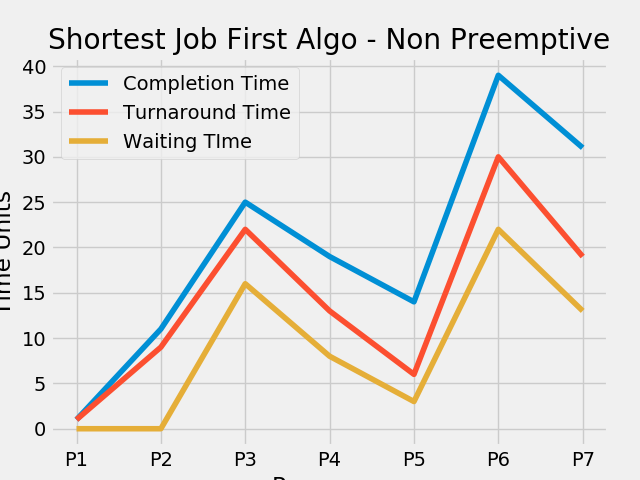
\includegraphics[scale=0.75]{./img/SJF_NP_output.png}
	\caption{SJF(Non-Preemptive) output values.}
\end{figure}}

{\begin{figure}[H]
	\centering
	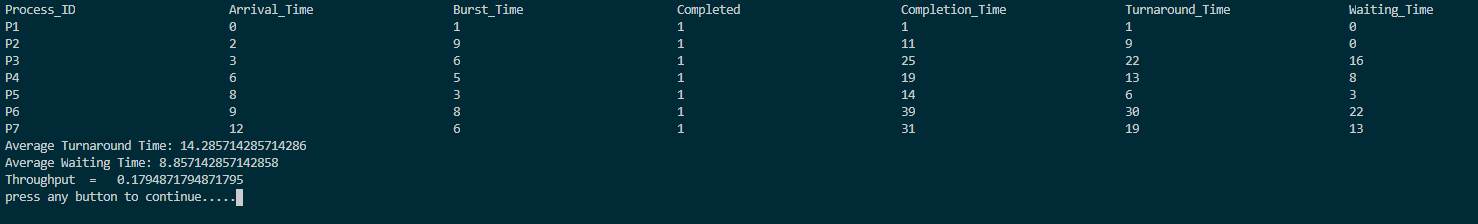
\includegraphics[scale=0.4]{./img/sjf_np_out.PNG}
	\caption{SJF(Non-Preemptive) output values.}
\end{figure}}


\chapter{Priorty Scheduling}
\section{Priorty(Preemptive)}
\begin{lstlisting}[columns=fullflexible,caption=Priority Scheduling Source Code,breaklines=true,postbreak=\mbox{\textcolor{red}{$\hookrightarrow$}\space},]
import matplotlib.pyplot as plt

plt.style.use('fivethirtyeight')


def schedulingProcess( process_data):
	start_time = []
	exit_time = []
	s_time = 0
	sequence_of_process = []
	process_data.sort(key=lambda x: x[1])
	'''
	Sort processes according to the Arrival Time
	'''
	while 1:
		ready_queue = []
		normal_queue = []
		temp = []
		for i in range(len(process_data)):
			if process_data[i][1] <= s_time and process_data[i][4] == 0:
				temp.extend([process_data[i][0], process_data[i][1], process_data[i][2], process_data[i][3],
								process_data[i][5]])
				ready_queue.append(temp)
				temp = []
			elif process_data[i][4] == 0:
				temp.extend([process_data[i][0], process_data[i][1], process_data[i][2], process_data[i][4],
								process_data[i][5]])
				normal_queue.append(temp)
				temp = []
		if len(ready_queue) == 0 and len(normal_queue) == 0:
			break
		if len(ready_queue) != 0:
			ready_queue.sort(key=lambda x: x[3], reverse=True)
			start_time.append(s_time)
			s_time = s_time + 1
			e_time = s_time
			exit_time.append(e_time)
			sequence_of_process.append(ready_queue[0][0])
			for k in range(len(process_data)):
				if process_data[k][0] == ready_queue[0][0]:
					break
			process_data[k][2] = process_data[k][2] - 1
			if process_data[k][2] == 0:       #if burst time is zero, it means process is completed
				process_data[k][4] = 1
				process_data[k].append(e_time)
		if len(ready_queue) == 0:
			normal_queue.sort(key=lambda x: x[1])
			if s_time < normal_queue[0][1]:
				s_time = normal_queue[0][1]
			start_time.append(s_time)
			s_time = s_time + 1
			e_time = s_time
			exit_time.append(e_time)
			sequence_of_process.append(normal_queue[0][0])
			for k in range(len(process_data)):
				if process_data[k][0] == normal_queue[0][0]:
					break
			process_data[k][2] = process_data[k][2] - 1
			if process_data[k][2] == 0:        #if burst time is zero, it means process is completed
				process_data[k][4] = 1
				process_data[k].append(e_time)
	calculateTurnaroundTime( process_data)
	calculateWaitingTime( process_data)
	twt = [p[8] for p in process_data]
	tat = [p[7] for p in process_data]
	ctime = [p[6] for p in process_data]
	return twt,tat,ctime,sequence_of_process

def calculateTurnaroundTime( process_data):
	total_turnaround_time = 0
	for i in range(len(process_data)):
		turnaround_time = process_data[i][6] - process_data[i][5]

		total_turnaround_time = total_turnaround_time + turnaround_time
		process_data[i].append(turnaround_time)



def calculateWaitingTime( process_data):
	total_waiting_time = 0
	for i in range(len(process_data)):
		waiting_time = process_data[i][6] - process_data[i][1]
		'''
		waiting_time = turnaround_time - burst_time
		'''
		total_waiting_time = total_waiting_time + waiting_time
		process_data[i].append(waiting_time)


def plot_graph(process_data):
	processes = [p[0] for p in process_data]
	twt = [p[8] for p in process_data]
	tat = [p[7] for p in process_data]
	ctime = [p[6] for p in process_data]

	plt.plot(processes,twt,label='Waiting Time')
	plt.plot(processes, tat, label = 'TurnAround Time')
	plt.plot(processes, ctime, label = 'Completion Time')

	plt.legend(loc='best')
	plt.savefig('./output/PRIORITY_P_output.png')
	plt.show()
	plt.close(fig='all')

def printData( process_data,sequence_of_process):
	process_data.sort(key=lambda x: x[0])
	'''
	Sort processes according to the Process ID
	'''
	print("Process_ID  Arrival_Time  Rem_Burst_Time   Priority        Completed  Orig_Burst_Time Completion_Time  Turnaround_Time  Waiting_Time")
	for i in range(len(process_data)):
		for j in range(len(process_data[i])):
			print(process_data[i][j], end='\t\t')
		print()
	print('\nAverage Turnaround Time:',sum(p[7] for p in process_data)/len(process_data))
	print('Average Waiting Time:',sum(p[8] for p in process_data)/len(process_data))
	print("Throughput: ",len(process_data)/max([p[6] for p in process_data]))
	print(f'Sequence of Process: {sequence_of_process}')



def priority_p():
	process_data = []
	with open('./inputs/PRIORITY_P.txt', 'r') as f:
		f.readline()
		for line in f.readlines():
			temporary = []
			process , burst , arrival,priority = (line.split(" "))
			temporary.extend([process, int(arrival), int(burst),int(priority), 0,int(burst)])
			process_data.append(temporary)

	sequence_of_process =  schedulingProcess( process_data)
	printData(process_data,sequence_of_process)
	plot_graph(process_data)

if __name__ == "__main__":
	priority_p()
\end{lstlisting}
{\begin{figure}[H]
	\centering
	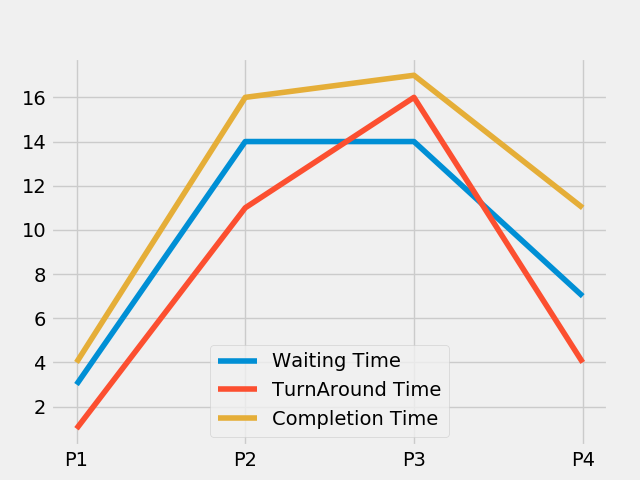
\includegraphics[scale=0.75]{./img/PRIORITY_P_output.png}
	\caption{Priority(Preemptive) output values.}
\end{figure}}

{\begin{figure}[H]
	\centering
	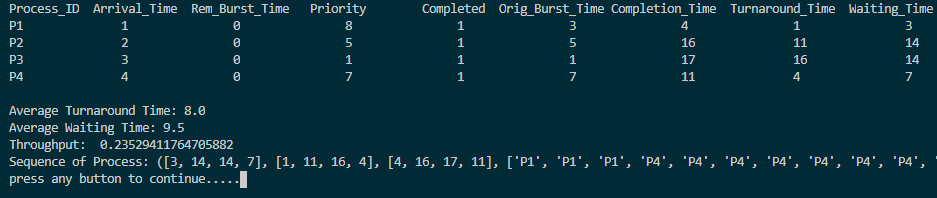
\includegraphics[scale=0.5]{./img/priority_p_out.PNG}
	\caption{Priority(Preemptive) output values.}
\end{figure}}

\section{Priorty(Non-Preemptive)}
\begin{lstlisting}[columns=fullflexible,caption=Priorty(Non-Preemptive) Source code,breaklines=true,postbreak=\mbox{\textcolor{red}{$\hookrightarrow$}\space},]
import matplotlib.pyplot as plt;

plt.style.use('fivethirtyeight')


def get_wt_time( wt, proc, totalprocess):  
	
	service = [0] * totalprocess
	
	service[0] = 0
	wt[0] = 0
	
	for i in range(1, totalprocess):  
		service[i] = proc[i - 1][1] + service[i - 1]  
		wt[i] = service[i] - proc[i][0] + 1
	
		if(wt[i] < 0) :      
			wt[i] = 0
			
def get_tat_time(tat, wt, proc, totalprocess):  
	
	for i in range(totalprocess): 
		tat[i] = proc[i][1] + wt[i]  
	
def findgc(proc, totalprocess): 
		
	wt = [0] * totalprocess
	tat = [0] * totalprocess
	wavg = 0
	tavg = 0
	get_wt_time(wt,proc, totalprocess)  
	get_tat_time(tat, wt, proc, totalprocess)  
	stime = [0] * totalprocess
	ctime = [0] * totalprocess
	stime[0] = 1
	ctime[0] = stime[0] + tat[0] 
	for i in range(1, totalprocess):  
		stime[i] = ctime[i - 1]  
		ctime[i] = stime[i] + tat[i] - wt[i]  

	for i in range(totalprocess): 
		wavg += wt[i]  
		tavg += tat[i]  

	return wt, tat,ctime


def print_details(processes,proc,arrival_time,ctime,tat,wt):
		
	print("Process_no\tStart_time\tComplete_time", 
				"\tTurn_Around_Time\tWaiting_Time\t\tPriority") 
	
	for i in range(len(processes)):
		print(proc[i][3], "\t\t", arrival_time[i],  
							"\t\t", end = " ") 
		print(ctime[i], "\t\t", tat[i], "\t\t\t", wt[i],'\t\t\t',proc[i][2])  
	
	print("Average waiting time is : ", end = " ") 
	print(sum(wt) / len(processes)) 
	print("average turnaround time : " , end = " ") 
	print(sum(tat) / len(processes)) 
	

def plot_graph(processes,wt,tat,ctime):

	plt.plot(processes, wt,label='Waiting Time')
	plt.plot(processes, tat, label = 'TurnAround Time')
	plt.plot(processes, ctime, label = 'Completion Time')

	plt.legend(loc='best')
	plt.savefig('./output/PRIORITY_NP_output.png')
	plt.show()
	plt.close(fig='all')


# Driver code  
def priority_np():

	processes = []
	burst_time = []
	arrival_time = []
	priority = []
	with open('./inputs/PRIORITY_NP.txt', 'r') as f:
		f.readline()
		for line in f.readlines():
			process, burst, arrival, prior = (line.split())
			processes.append(process)
			burst_time.append(int(burst))
			arrival_time.append(int(arrival))
			priority.append(int(prior)) 
	

	totalprocess = len(processes)
	proc = []
	for i in range(totalprocess): 
		l = [] 
		for j in range(4): 
			l.append(0) 
		proc.append(l) 
	
	
	for i in range(totalprocess):
		proc[i][0] = arrival_time[i]
		proc[i][1] = burst_time[i]
		proc[i][2] = priority[i]
		proc[i][3] = processes[i]

	proc = sorted (proc, key = lambda x:x[2]) 
	proc = sorted (proc) 
	wt, tat,ctime = findgc(proc,totalprocess) 
	print_details(processes,proc,arrival_time,ctime,tat,wt)
	plot_graph(processes,wt,tat,ctime)
	plt.close(fig='all')
	


if __name__ =="__main__": 
	priority_np()
	
\end{lstlisting}

{\begin{figure}[H]
	\centering
	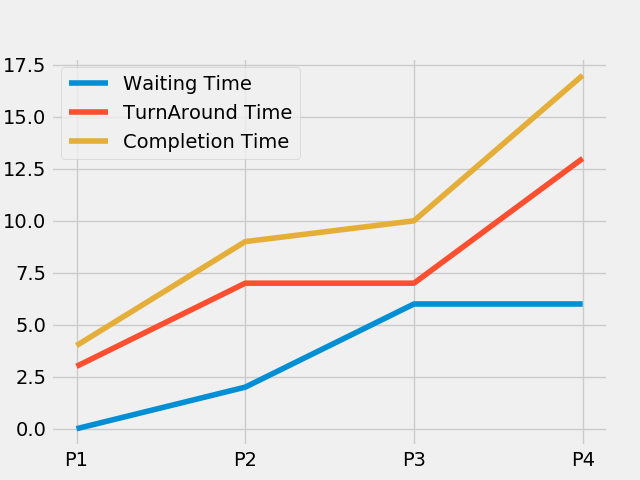
\includegraphics[scale=0.75]{./img/PRIORITY_NP_output.png}
	\caption{Priority(Non-Preemptive) output values.}
\end{figure}}

{\begin{figure}[H]
	\centering
	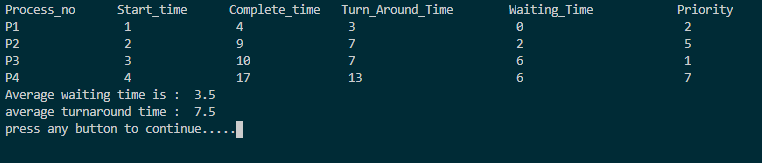
\includegraphics[scale=0.75]{./img/priority_np_out.PNG}
	\caption{Priority(Non-Preemptive) output values.}
\end{figure}}

\chapter{Round Robin}
\begin{lstlisting}[columns=fullflexible,caption = Round Robin Source Code,breaklines=true,postbreak=\mbox{\textcolor{red}{$\hookrightarrow$}\space},]
import matplotlib.pyplot as plt
from statistics import mean

plt.style.use('fivethirtyeight')



def findWaitingTime(processes, n, burst_time, waiting_time, quantum):  
    rem_burst_time = [0] * n 

    for i in range(n):  
        rem_burst_time[i] = burst_time[i] 
    t = 0
    while(1): 
        done = True
        for i in range(n): 
            if (rem_burst_time[i] > 0) : 
                done = False 
                  
                if (rem_burst_time[i] > quantum) : 
                    t += quantum  
                    rem_burst_time[i] -= quantum  
                else: 
                    t = t + rem_burst_time[i]  
                    waiting_time[i] = t - burst_time[i]  
                    rem_burst_time[i] = 0
        if (done == True): 
            break
              

def findTurnAroundTime(processes, n, burst_time, waiting_time, tat): 
    for i in range(n): 
        tat[i] = burst_time[i] + waiting_time[i]  
  
  

def findavgTime(processes, n, burst_time,arrival_time, quantum):  
    waiting_time = [0] * n 
    tat = [0] * n  
    compl_time = [0]*len(processes)

    findWaitingTime(processes, n, burst_time,  waiting_time, quantum)  

    findTurnAroundTime(processes, n, burst_time, waiting_time, tat)    
    total_waiting_time = 0
    total_tat = 0
    for i in range(n): 
        total_waiting_time = total_waiting_time + waiting_time[i]  
        total_tat = total_tat + tat[i]  
        compl_time[i] = arrival_time[i] + tat[i]
    return waiting_time, tat ,compl_time
      


def plot_graph_normal(processes,waiting_time,compl_time,turn_around_time,ax1):
    
    ax1.plot(processes,waiting_time,label = "waiting_time")
    ax1.plot(processes,compl_time,label = "Completion time")
    ax1.plot(processes,turn_around_time,label = "Turnaround Time")

    ax1.legend()
   # plt.savefig('../output/ROUND_ROBIN_output.png')


def plot_graph_quantum(processes, burst_time, arrival_time,ax2):
    throughput_quantum = []
    avg_waiting_quantum = []
    avg_turnaround_quantum = []
    avg_completion_quantum =[]
    for n in range(1,10):
        waiting_time,turn_around_time,compl_time =  findavgTime(processes, len(processes), burst_time, arrival_time, n) 
        throughput_quantum.append(len(processes)/ compl_time[len(processes)-1])
        avg_turnaround_quantum.append(mean(turn_around_time))
        avg_completion_quantum.append(mean(compl_time))
        avg_waiting_quantum.append(mean(waiting_time))

    rang = list(range(1,10))
    ax2.plot(rang,throughput_quantum,label="Throughput")
    ax2.plot(rang,avg_waiting_quantum,label="Average waiting_time")
    ax2.plot(rang,avg_completion_quantum,label="Average Completion Time")
    ax2.plot(rang,avg_turnaround_quantum,label="Average Turn Around Time")

    ax2.legend()



def print_details(processes,burst_time,waiting_time,compl_time,tat):
    print("Processes    Burst Time     Waiting  Time    Turn-Around Time    Completion Time") 
    for i in range(len(processes)):
           print(" ", processes[i] , "\t\t", burst_time[i], "\t\t", waiting_time[i], "\t\t", tat[i],"\t\t",compl_time[i]) 
    print("\nAverage waiting_time = %.5f "%(sum(waiting_time) /len(processes)) ) 
    print("Average turn around time = %.5f "% (sum(tat) / len(processes)))  
    print('Throughput = ', len(processes)/ max(compl_time))
    print('Average Job elapsed time = ',sum(tat)/len(processes))



def round_robin():
    f, (ax1, ax2) = plt.subplots(1, 2, sharey=True)
    processes = []
    burst_time = []
    arrival_time = []
    #breakpoint
    with open('./inputs/ROUND_ROBIN.txt','r') as  f:
        f.readline()
        for line in f.readlines():
            process , burst , arrival = (line.split(" "))
            processes.append(process)
            burst_time.append(int(burst))
            arrival_time.append(int(arrival))


    # Time quantum  
    quantum = 2;  
    waiting_time,turn_around_time,compl_time =  findavgTime(processes, len(processes), burst_time, arrival_time, quantum) 
    print_details(processes,burst_time,waiting_time,compl_time,turn_around_time)
    plot_graph_normal(processes,waiting_time,compl_time,turn_around_time,ax1)
    plot_graph_quantum(processes, burst_time, arrival_time,ax2)
    plt.savefig("./output/ROUND_ROBIN.png")
    plt.show()
    plt.close(fig='all')

# Driver code  
if __name__ =="__main__": 
      round_robin()

  
\end{lstlisting}
\begin{figure}[H]
	\centering
	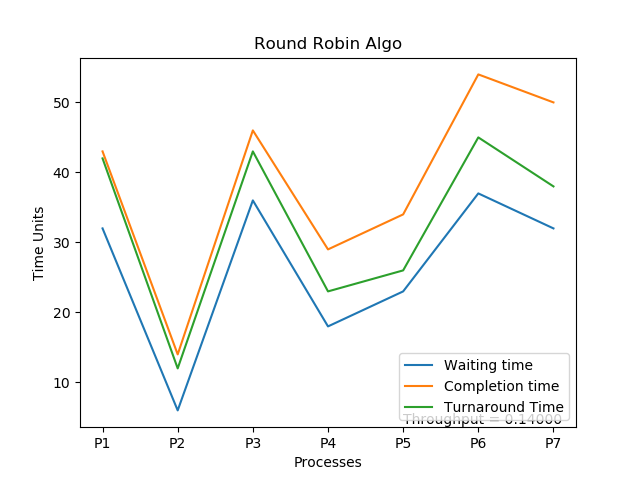
\includegraphics[scale=0.8]{./img/ROUND_ROBIN_output.png}
	\caption{Round Robin output values.}
\end{figure}

\begin{figure}[H]

	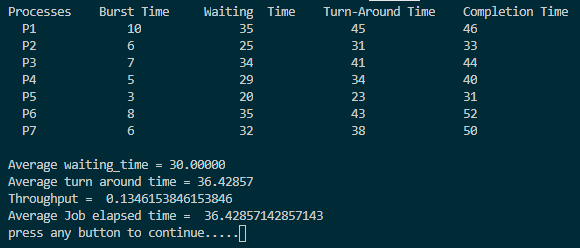
\includegraphics[scale=0.9]{./img/rr_out.PNG}
	\caption{Round Robin output values.}
\end{figure}


\begin{figure}[H]

	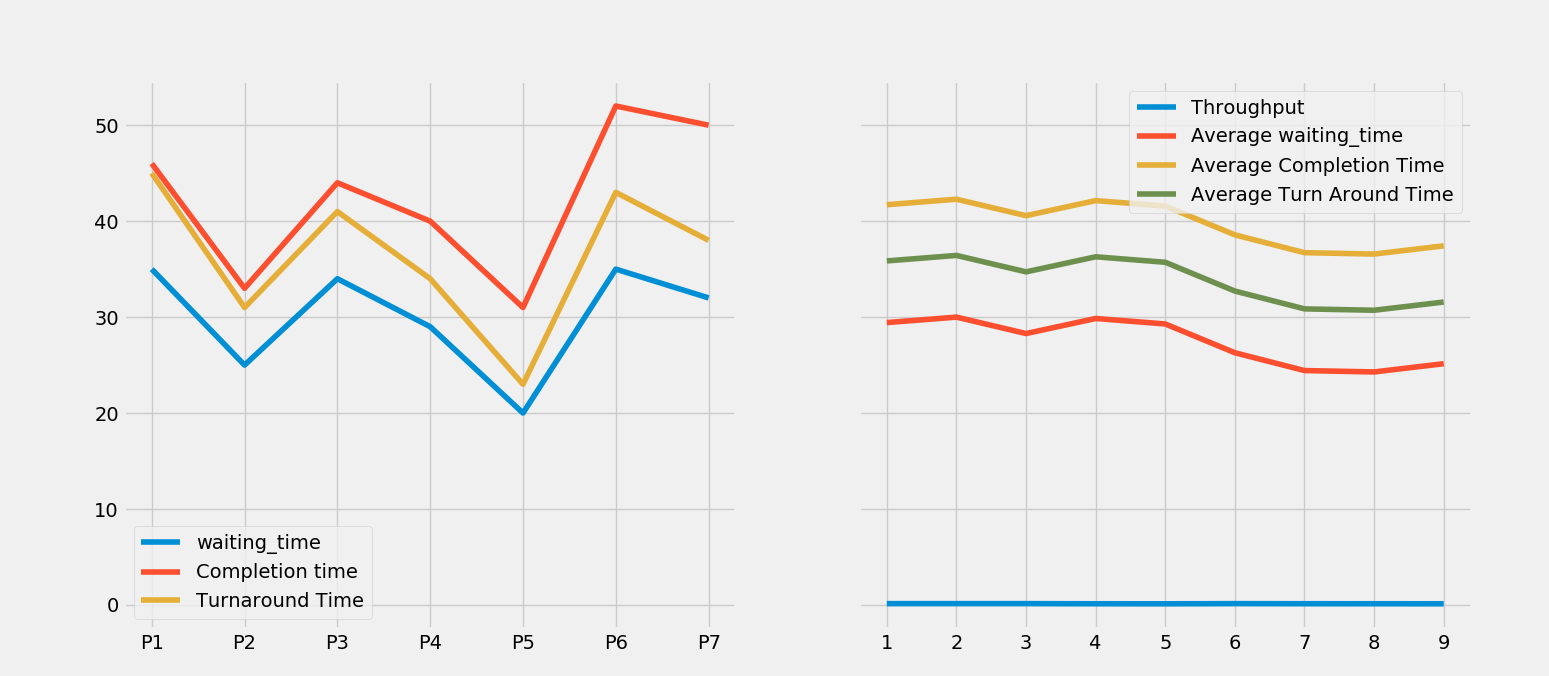
\includegraphics[scale=0.4]{./img/ROUND_ROBIN.png}
	\caption{Round Robin (per quantum) output values.}
\end{figure}




\chapter{Conclusion}
\vskip 1cm
\hspace*{\parindent}From the given project work we have concluded that the difference between the turn around time,average waiting time,average elapsed time and completion time for same input of different cpu scheduling is as follows:-
\vskip 1cm
\begin{figure}[H]
	\centering
	\includegraphics[scale=0.9]{./img/compare.png}
	\caption{comparison between CPU scheduling.}
\end{figure}
\vskip 1cm
From the above graph we came to know that every algorithm works better on the significant problem as the fcfs is better for a small burst time.The sjf is better if the process comes to processor simultaneously and round robin, is better to adjust the average waiting time desired and the priorty works better  where the relative important of each process may be precisely defined.

\vskip 15cm

\chapter{References}
\vskip 1cm
{\subsection*{}
The source code of the project can be found at:-\\
	\url{https://github.com/cannibalcheeseburger/cpu-scheduling-simluation.git}\\
And the other references we used for this project are given:-
\begin{itemize}
\item 	A. Dusseau, R. H. dan A. C., Operating Systems: Three Easy Pieces, Arpaci-Dusseau Books, 2014.
\item Operating System Principles – Galvin
\item Tanenbaum, Modern Operating Systems, Pearson Education, Inc., 2008.
\item 	\url{http://www.cs.uic.edu/~jbell/CourseNotes/OperatingSystems/5_CPU_Scheduling.html}
\item \url{http://codex.cs.yale.edu/avi/os-book/OS8/os8c/slide-dir/PDF-dir/ch5.pdf}
\end{itemize}

}

\end{document}